\documentclass[12pt,a4paper]{article}
\usepackage[UTF8]{ctex}
\usepackage{amsmath,amssymb}
\usepackage{xcolor}
\usepackage{hyperref}
\usepackage{geometry}
\usepackage{graphicx}
\geometry{margin=2.5cm}

\title{BB84 Quantum Key Distribution}
\author{QuoNic}
\date{}

\begin{document}
\maketitle

\begin{center}
\textbf{Communication} | Difficulty: Intermediate | Time: 15 min
\end{center}

\tableofcontents
\newpage

\section{Why do we need it?}

BB84 is the first quantum key distribution protocol, using quantum mechanics for unconditionally secure key distribution.

\subsection{Classical Limitations}
\begin{itemize}
  \item Classical encryption relies on computational complexity (e.g., RSA)
  \item Quantum computers can break classical encryption
  \item Classical key distribution requires trusted channel
\end{itemize}

\subsection{Quantum Advantages}
\begin{itemize}
  \item BB84 provides information-theoretic security (no computational complexity)
  \item No-cloning theorem ensures eavesdropping detection
  \item Foundation for post-quantum cryptography
\end{itemize}

\subsection{Real-world Applications}
\begin{itemize}
  \item Quantum Key Distribution networks
  \item Quantum secure communication
  \item Quantum internet
\end{itemize}

\section{Quick Start}

\begin{verbatim}
from quonic.algorithms import bb84

# Run BB84 protocol
result = bb84(n_bits=100, noise=0.0)
print(f"Shared key: {result.key}")
print(f"Key length: {len(result.key)}")
\end{verbatim}

\textbf{Expected Output}:
\begin{verbatim}
Shared key: 01101001...
Key length: 50
\end{verbatim}

\section{Theory Deep Dive}

\subsection{Circuit Diagram}

\begin{center}
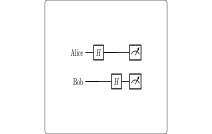
\includegraphics[width=0.5\textwidth]{../../images/bb84_circuit.svg}
\end{center}

\subsection{Mathematical Derivation}

BB84 protocol steps:
\begin{enumerate}
  \item Alice randomly chooses bits and bases
  \item Alice prepares quantum states and sends to Bob
  \item Bob randomly chooses bases to measure
  \item Alice and Bob publicly compare bases
  \item Keep bits where bases match as key
\end{enumerate}

Security based on no-cloning theorem:
\begin{equation}
|\psi\rangle \neq |\phi\rangle \Rightarrow \text{cannot perfectly clone}
\end{equation}

\subsection{Geometric Interpretation}

On the Bloch sphere, BB84 uses two orthogonal bases:
\begin{itemize}
  \item Computational basis: $\{|0\rangle, |1\rangle\}$
  \item Hadamard basis: $\{|+\rangle, |-\rangle\}$
\end{itemize}

Eavesdropper doesn't know Alice's basis, measurement introduces errors.

\section{Code Walkthrough}

\begin{verbatim}
from quonic.algorithms import bb84

# bb84(n_bits, noise)
# n_bits: number of bits to generate
# noise: channel noise rate
result = bb84(n_bits=100, noise=0.0)

# result.key: shared secret key
# result.error_rate: quantum bit error rate
print(f"Key: {result.key}")
print(f"Error rate: {result.error_rate}")
\end{verbatim}

\section{Advanced Usage}

\subsection{Scenario 1: Noisy BB84}

\begin{verbatim}
# BB84 with channel noise
result = bb84(n_bits=100, noise=0.05)
print(f"Error rate: {result.error_rate}")
# If error rate > 11%, channel may be compromised
\end{verbatim}

\subsection{Scenario 2: Eavesdropping Detection}

\begin{verbatim}
# Eavesdropping detection
result = bb84(n_bits=100, noise=0.0)
if result.error_rate > 0.11:
    print("Eavesdropper detected!")
else:
    print("Channel is secure")
\end{verbatim}

\section{Use Cases}

\subsection{Quantum Key Distribution Networks}

BB84 can be used to build quantum key distribution networks for secure communication.

\subsection{Quantum Secure Communication}

BB84 provides information-theoretic security for high-security communication needs.

\subsection{Quantum Internet}

BB84 is one of the foundational protocols for the quantum internet.

\section{FAQ}

\subsection{Why is BB84 secure?}

BB84 security is based on the no-cloning theorem. Eavesdroppers cannot perfectly clone quantum states, and measurement introduces errors.

\subsection{What is the key generation rate of BB84?}

Ideally, BB84 key generation rate is about 50\% (probability of basis matching).

\subsection{Can BB84 resist quantum computers?}

BB84 provides information-theoretic security, not relying on computational complexity, so it can resist quantum computers.

\section{Learning Path}

\subsection{Prerequisites}
\begin{itemize}
  \item Qubits and superposition
  \item Hadamard gate and measurement
  \item No-cloning theorem
\end{itemize}

\subsection{Next Steps}
\begin{itemize}
  \item E91 Protocol (entanglement-based QKD)
  \item Quantum Repeaters
  \item Quantum Internet
\end{itemize}

\section{Complete Examples}

\subsection{Example 1: Basic BB84}

\begin{verbatim}
from quonic.algorithms import bb84

result = bb84(n_bits=100, noise=0.0)
print(f"Key: {result.key}")
\end{verbatim}

\section{Download}

\begin{itemize}
  \item [bb84.py](https://github.com/ChrisLee0721/QuoNic/blob/main/examples/bb84/bb84.py)
\end{itemize}

\end{document}
